\subsection{Transparenz durch das gewählte Modell}
Einige ML-Algorithmen gelten als in sich transparent. So liegt es auf der Hand, dass diese für transparentes ML eingesetzt werden können. 
Abbildung \ref{Fig:interpretierbarkeitJeModell} gibt einen guten Überblick, welche dabei hilft einzuordnen, ob ein Algorithmus leicht von Menschen verstanden werden kann.
\begin{figure}
    \centering
    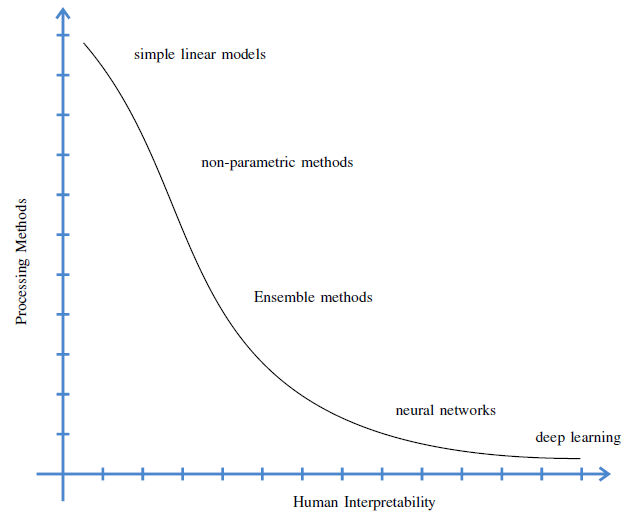
\includegraphics[scale=0.55]{pic/MA-Bilder/Literaturrecherche/48-InterpretierbarkeitJeModell.PNG}
    \caption{Interpretierbarkeit je nach Modell, entnommen aus: \cite{vorm2018assessing}}
    \label{Fig:interpretierbarkeitJeModell}
\end{figure}

\subsubsection{Transparente Modelle}
\label{subsubsec_transparenteModelle}
Folgend wird aufgelistet, welche Methoden als transparent gelten mit Bezug auf die jeweiligen Quellverweise.
\begin{itemize}
    \item Lineare Regression \cite{hanif2021survey, chen2021novel, palaniyappan2022aqx, ribeiro2016should}
    \item Logistische Regression \cite{hanif2021survey, schoeffer2022human, krause2017workflow, palaniyappan2022aqx, hill2018balancing}
    \item Entscheidungsbäume \cite{hanif2021survey, chen2021novel, krause2017workflow, de2018algorithmic, palaniyappan2022aqx}
    \item Random Forest \cite{chen2021novel, ribeiro2016should}
    \item Entscheidungsregeln (Wenn-Dann-Aussagen) \cite{hanif2021survey, chen2021novel}
    \item Generalized Linear Models (GLM) \cite{hanif2021survey}
    \item Generalized Linear Rules \cite{hanif2021survey}
    \item Generalized Additive Models (GAMs) \cite{hanif2021survey}
    \item Bayesche Regeln \cite{de2018algorithmic}
    \item k-nächste Nachbarn \cite{palaniyappan2022aqx}
\end{itemize}

In Bezug auf transparente Modelle sei angemerkt, dass einige dieser Methoden teilweise transparenter sind als andere. So geben \cite{hill2018balancing} an, dass logistische Regression leichter nachzuvollziehen sei als Random Forest, wenngleich Random Forests bessere Ergebnisse liefern. Ein weiterer wichtiger Aspekt ist, dass transparente Modelle (konkret von den Autoren genannt: logistische Regression und Entscheidungsbäume) zwar transparent seien, aber schwer zu generalisieren sind.

Daneben existieren noch weitere Ansätze von Wissenschaftlern, welche ihre eigenen transparenten Modelle entwickeln. Diese basieren jedoch meistens auf den Mechanismen, welche sich in den Methoden der obigen Listen wiederfinden lassen. 
Ein Beispiel für ein solches Modell sind fast-and-frugal-trees \cite{keller2020augmenting}, dessen Funktionsweise auf Entscheidungsbäumen basiert. Als besonderer Vorteil wird hier von den Autoren genannt, dass sich diese Art von Bäumen leicht visualisieren lässt und kein Hinzufügen nachträglicher Erklärungen (wie es bei Post-Hoc-Methoden der Fall ist) nötig ist. Somit ist eine Entwicklung mit einer solchen Methode zusätzlich weniger aufwendig.
Auch \cite{ainon2009transparent} entwickelten ein eigenes transparentes Klassifikationsmodell, indem sie mehrere transparente Methoden kombinieren, z.B. neuronale Netze und Wenn-Dann-Regeln. Diese erlauben eine transparente Abbildung des neuronalen Netzes. Dieses ist streng genommen keine neue Methode, sondern eine Anwendung von Global Surrogate \todo[inline]{Todo: Referenz auf Abschnitt im Kapitel der XAI-Methoden}

% das verstehe ich leider nicht: \cite{wang2005novel} eigene transparente Methode: feature decomposition method